:\subsection{Raspberry Pi Camera}
\begin{figure}[h]
    \centering
    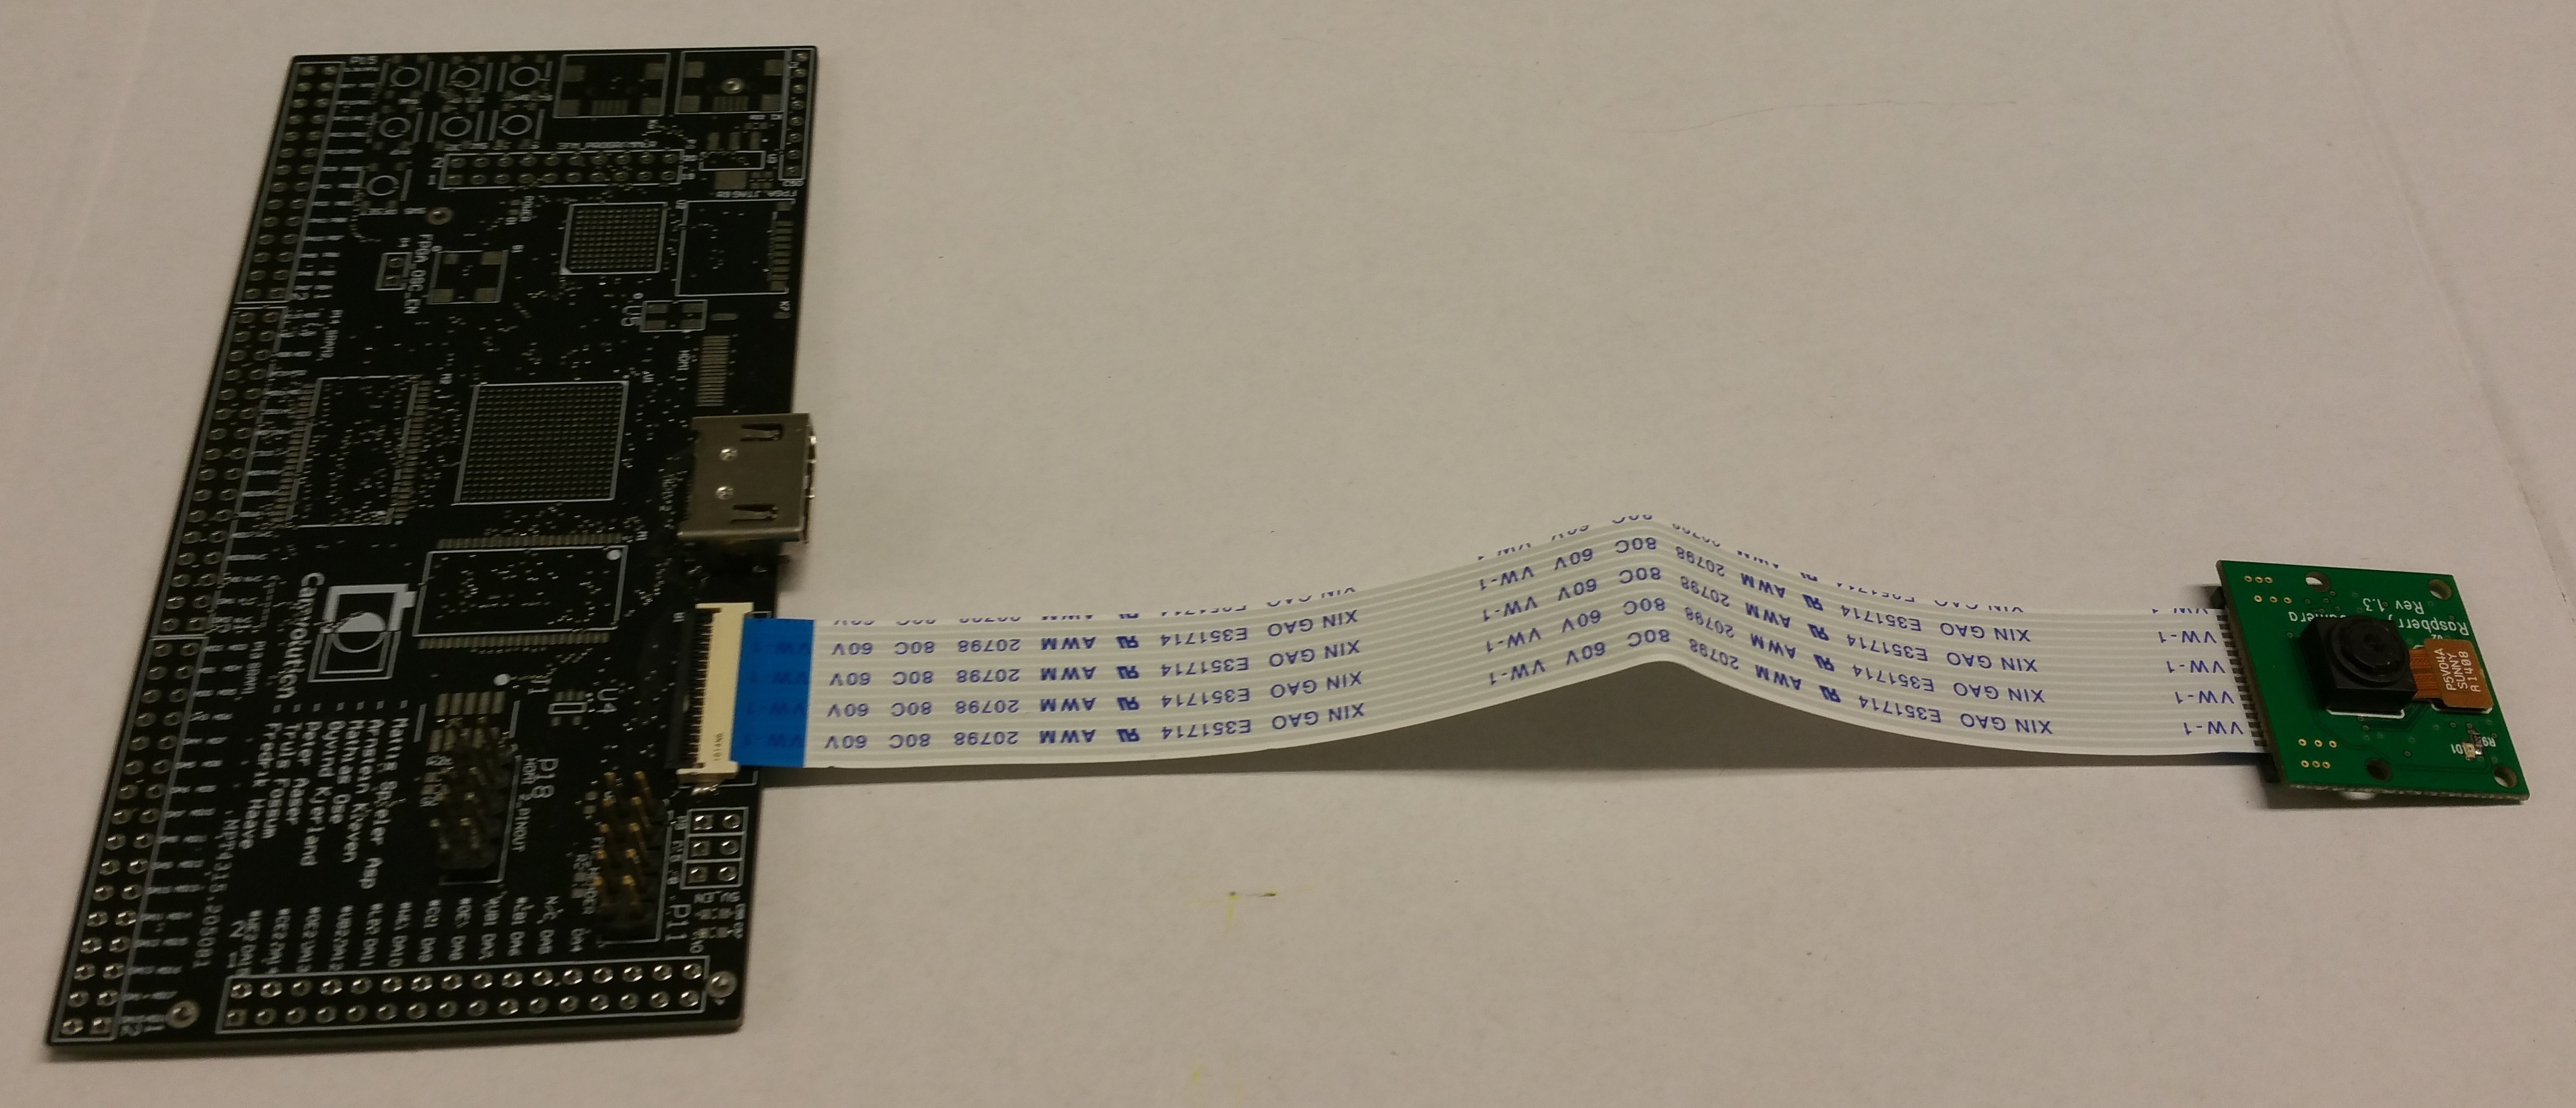
\includegraphics[width=0.75\textwidth]{img/picamera}
    \caption{Raspberry Pi Camera}
\end{figure}

The \textit{Raspberry Pi Foundation} has designed this peripheral for use with the \textit{Raspberry Pi} computer.
The PiCamera can take still shots as well as record continuous video.
The module consists of a camera sensor on a board with a controller unit which connects to the Pi (or another master device) via a 16-pin ribbon cable.
Communication over this cable is defined by the proprietary \textit{MIPI Camera Serial Interface} (CSI) specification.

The master device controls the camera module by sending instructions over an I2C bus on the ribbon cable,
and the camera module responds with picture data over two clocked differential busses.
Parameters that may be controlled include video encoding, resolution in two dimensions and framerate.

